%! Author = mariuszindel
%! Date = 25.01.21

\section{Abtasten}

\subsection{Abtasttheorem}
Damit keine Spektrumsüberlappungen (engl. Aliasing) beim Abtasten auftreten, muss die zweiseitige Bandbreite B des abzutastenden Signals kleiner als die Abtastfrequenz $f_s$
sein.\\
Dies bedeutet, dass die grösste im Spektrum vorkommende Frequenz kleiner als die Hälfte der Abtastfrequenz sein muss.\\
$B<f_s$ oder $f_{max} < f_s / 2$

\subsection{Abgetasteter zeitdiskreter Reckteckpuls}
\begin{center}
    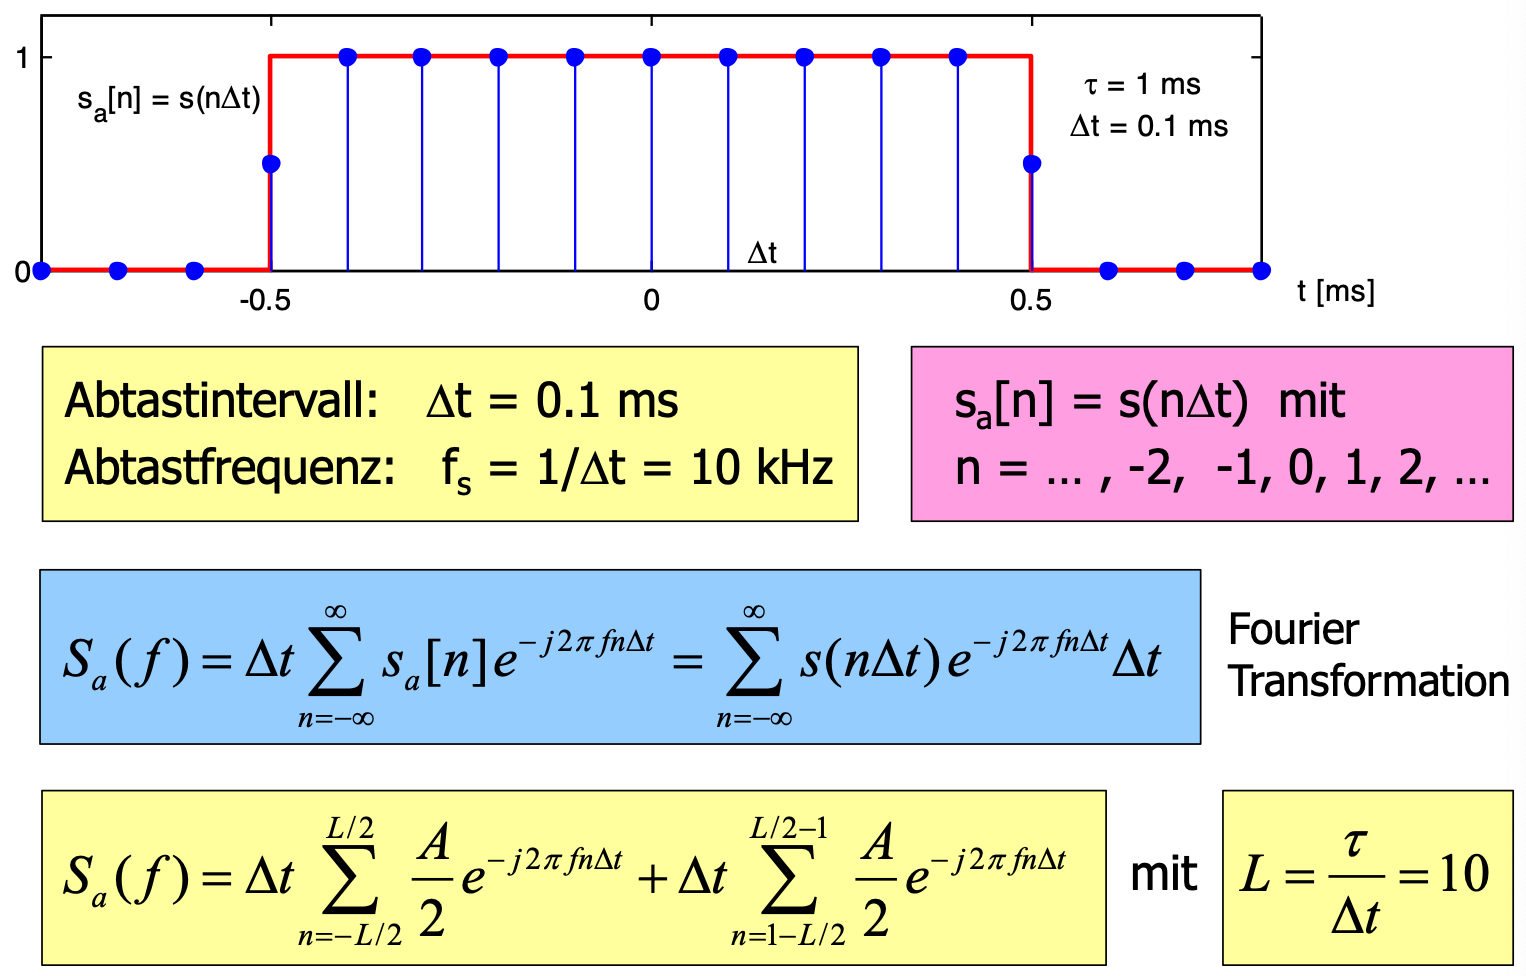
\includegraphics[width=\linewidth]{graphic/sprache-digitalisieren/Abgetasteter zeitdiskreter Reckteckpuls.png}
\end{center}
\vspace{-8pt}
Was bewirkt die gezielte Wahl der Smapling Frequenz $f_s = f_0$? Antwort: Das Sampling mit der Trägerfrequenz $f_0$ bewirkt eine Verschiebung des Datensignals in das Basisband und damit eine Produktdemodulation mit $f_0$.


\subsection{Aliasing}
Damit Frequenzkomponenten, die Aliasing verursachen, genügend unterdrückt werden können, muss die Grenzfrequenz $f_g$des Tiefpassfilters ca. 10\% unter derhalben Abtastfrequenz $f_s/ 2$ liegen.
$\rightarrow$ Aliasing tritt auf, wenn im abzutastenden Signal Frequenzanteile vorkommen, die höher sind als die halbe Abtastfrequenz. $Signal > 1/2 \times Abtastfrequenz$. Durch vorschalten eines Tiefpassfilters mit einer Grenzfrequenz $f_g < f_s / 2$, kann Aliasing vermieden werden.
\vspace{-8pt}
\begin{center}
    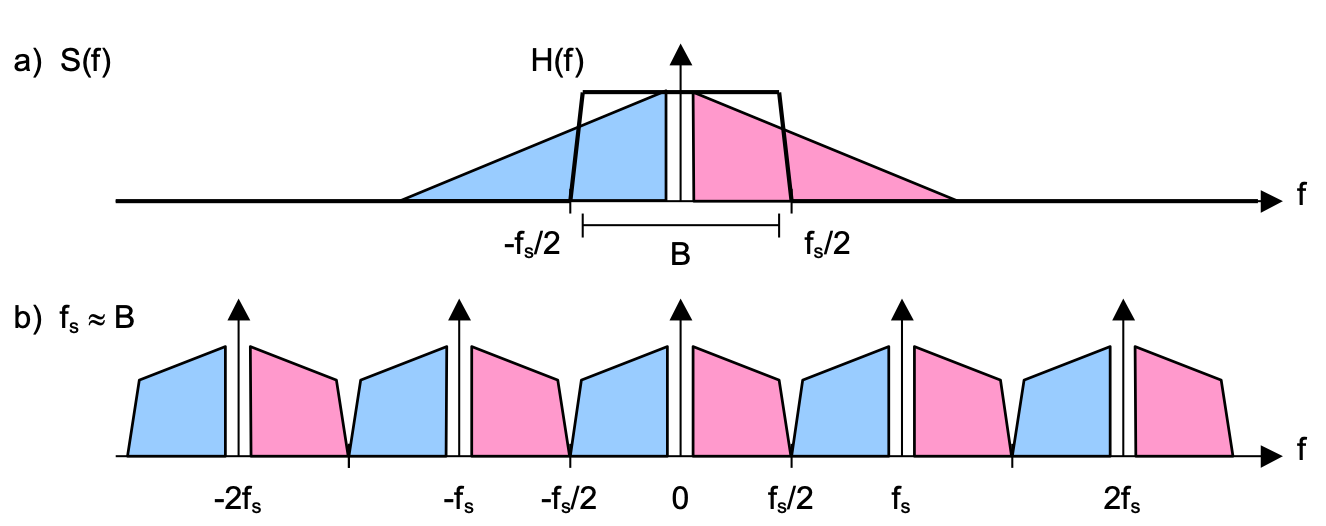
\includegraphics[width=\linewidth]{graphic/sprache-digitalisieren/Aliasing.png}
\end{center}
\vspace{-8pt}

